%
%	Praxisbezug
%

\pagebreak
\section{Using Rancher as an Enterprise Container Management Platform}

\onehalfspacing

\subsection{Rancher overview}

What is Rancher? According to the Rancher Labs website, it is "[...] a complete software stack for teams adopting containers. It addresses the operational and security challenges of managing multiple Kubernetes clusters, while providing DevOps teams with integrated tools for running containerized workloads"\footnote{\textit{Rancher Labs (2019)}: Run Kubernetes Everywhere. \cite{rancher}}

Rancher provides a management platform to centrally manage multiple Kubernetes clusters in Enterprise IT, all from a user-friendly GUI. Rancher also offers integration tools for application development and robust enterprise-grade features for security and governance. For operations, Rancher provides integrated solutions for logging, monitoring, and auditing, amongst other features.

Gartner recognized Rancher Labs in 2019 as a Firestarter in Gartner's annual technology award program.\footnote{See \textit{Rancher Labs (2019)}: Rancher Labs Recognized by 451 Research as a ‘451 Firestarter’. \cite{firestarter451}}

Rancher Labs offers many more open-source projects besides Rancher. There's RIO, a toolchain to streamline application development and deployment, and K3s, the Kubernetes distribution for edge computing. Rancher Labs funds itself solely through revenues from support, training, and consulting; they are not following a freemium or core approach, as many other open-source businesses do.

\subsection{Rancher GUI}

The central element of Rancher is the GUI provided by the Rancher server itself. It offers one-stop access for all administrative tasks necessary on Kubernetes clusters, from installation, upgrading, and decommissioning to hardening. The GUI allows all application administration, and also offers easy access to troubleshooting information. For developers, it provides user authentication and pipeline connection.

Let's look at an example. The Rancher Dashboard for an active Kubernetes cluster looks like this:

\begin{figure}[H]
\centering
\caption {Rancher Dashboard}
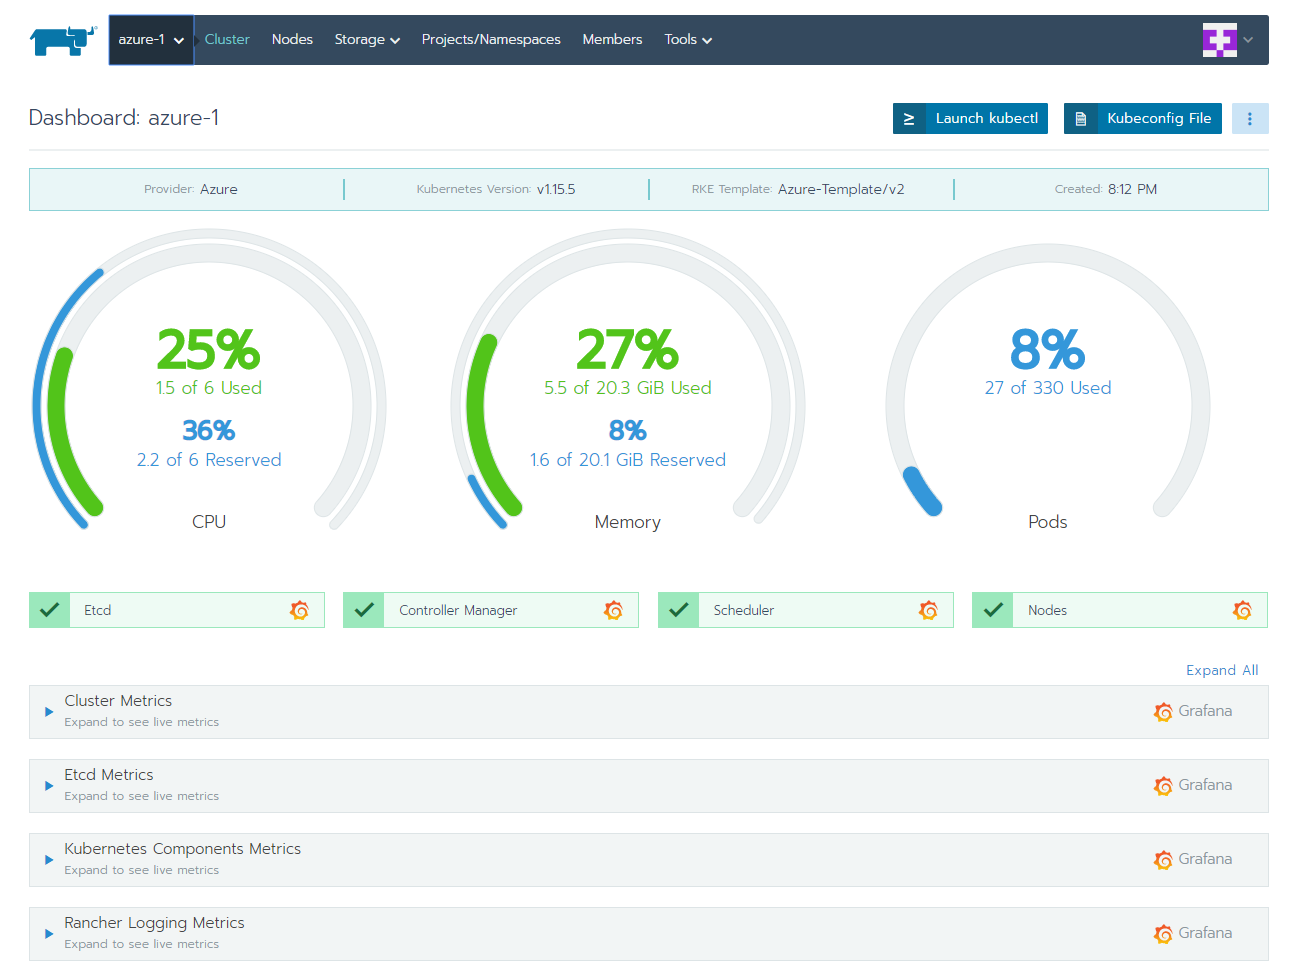
\includegraphics[width=\linewidth]{images/dashboard}
\label{fig:rancherDashboard}
\end{figure}

This cluster was created on Azure and has cluster monitoring enabled. At a glance we can see that CPU utilization is at 25\%, memory utilization is at 27\%, and 27 out of 330 possible pods are running; we can also see the Kubernetes version installed (v1.15.5), the cluster template used and the date and time the cluster was created.

The cluster dashboard gives an overview of the overall health of the cluster, including the event stream - a similar, more detailed panel is available for all deployed applications. This information is available for all clusters in a consistent manner, regardless of whether they're hosted on a public cloud provider or in-house. Access to the dashboard is based on user permissions, of course.

From the dashboard, all administrative tasks can be performed by drilling down on the individual components that make up the cluster and are present in the GUI, nodes, volumes, and applications.

\subsection{Rancher Architecture}

Rancher is, similar to Kubernetes, itself a containerized application and can be installed from a single image to a single Docker host. Such a single-node installation is ideal for testbeds or local Rancher installations on a laptop, for example. A single node installation does not provide any redundancy in case of failure.

For production installations, Rancher can be installed on a Kubernetes cluster, using Kubernetes' redundancy mechanisms for high-availability and resiliency. It could either be co-hosted on an existing cluster or better, on a small, separate infrastructure cluster. It is good practice in IT to keep administrative tools on separate infrastructure from the administered infrastructure, and thus the installation on a different cluster is the most widespread.

In addition to the GUI, the Rancher server also provides a central Kubernetes API endpoint, which acts as an intermediary between the users and the actual Kubernetes clusters.

Rancher too has a command-line interface tool, rancher, to access the API; a detailed description can be found in the Rancher online documentation.\footnote{See \textit{Rancher Labs (2019)}: Using the Rancher Command Line Interface. \cite{rancherCLI}}

\subsection{Authentication and Authorization}

Acting as an intermediary, Rancher can centrally authenticate user logins, and API calls through a variety of identity providers, most commonly with Microsoft's Active Directory. Once the user is authenticated, Rancher introduces a new level of hierarchy to Kubernetes, the Project.

Projects on a cluster can include Kubernetes namespaces, workloads or applications and serve as a logical group for teams or applications. 

Rancher includes a variety of predefined roles, that can be easily expanded to match any organizational needs.

These roles, and the permissions that come with the roles, can then be assigned to one or many users or groups, on cluster or project/application level, providing fine-grained central role-based access control for all connected Kubernetes clusters.

This authentication and authorization mechanism works for the GUI, the Rancher CLI, or any other Rest-API Call to the Rancher server.

\subsection{Security Policies}

Kubernetes provides Pod Security Policies and Network Policies, at the cluster level. The Rancher GUI allows to manage these policies from a central interface and apply them uniformly to all managed clusters; managing these policies from a graphical interface is also much less error-prone than writing YAML files and distributing them manually.

In addition to policies, Rancher provides templates for cluster and node creation that can help to ensure organizational compliance and common security standards. For cluster hardening, Rancher provides a detailed, easy to follow hardening guide.\footnote{See \textit{Rancher Labs (2019)}: Hardening Guide - Rancher v2.3.x. \cite{hardeningGuide}}

\subsection{Cluster Management}

From these templates, the installation of a new cluster through the GUI is quite simple and accomplished with a few clicks. Rancher provides cluster drivers for managed Kubernetes on the three major public cloud providers (Google GKE, Amazon EKS, and Microsoft Azure AKS) and node drivers for the same, plus several infrastructure providers, including VMware.

As of the latest Rancher version (2.3.3), the VMware node driver now supports dynamic provisioning of worker nodes so that fully flexible and breathing clusters can be implemented on an in-house ESXi cluster farm; previously, this feature was limited to public cloud infrastructure.

Clusters provisioned and installed through Rancher can also be upgraded through the Rancher GUI with a single click. Once a new version has been selected, Rancher will perform a rolling upgrade of all master and worker nodes, without application downtime.

For application management, Rancher interacts with the popular package manager Helm.\footnote{See \textit{CNCF (2019)}: Helm 3 - The package manager for Kubernetes. \cite{helm}} Helm is also used as the base installation mechanism for Rancher's integrated application catalogs, which can be extended.

Helm, directly or through the catalogs, provides version control and upgrades for application deployments.

\subsection{Logging and Monitoring}

From the GUI, Logging can be defined for each cluster. Several log drivers are included out-of-the-box, from the venerable Syslog to the more modern Elasticsearch;\footnote{See \textit{Elasticsearch (2019)}: The heart of the Elastic Stack. \cite{elastic}} Rancher will fully install and configure log forwarders and make sure that the log records are complete.

If so desired, Rancher can install and configure a Prometheus monitoring instance with pre-configured Grafana dashboards on each cluster;\footnote{See \textit{The Linux Foundation (2019)}: From metrics to insight. \cite{prometheus}} \footnote{See \textit{Grafana Labs (2019)}: The open observability platform. \cite{grafana}} the Grafana dashboards for cluster and application monitoring are all accessible from the Rancher GUI.

\subsection{Backup and restore}

Configuration and state of a Kubernetes cluster are stored in a distributed key-value store. For clusters provisioned by Rancher, Rancher can provide regularly scheduled backups of this datastore, either locally or to an S3-compliant object store; Rancher also offers the functionality to restore such snapshots from the GUI.

\subsection{Persistent volumes}

For persistent data storage, Kubernetes can provide volume mounts to application pods via the deployment definition. The available classes of volumes are dependent on the underlying infrastructure provider and the installed storage classes.

Rancher offers the creation and management of persistent volumes from the GUI.

Rancher does not offer backup and restore services for these volumes, though.

\subsection{CI/CD}

For application development, Rancher can install and configure a complete CI/CD pipeline from the GUI on a given cluster; the pipeline is based on Jenkins and can connect to all major source-code revision control systems.

Good software development practice calls for credentials to be stored apart from source code. Kubernetes offers secrets as objects for this purpose and has a built-in secret store. Rancher also has an integrated secret store, with significantly higher encryption and improved access control.

It is also good practice to separate code and configuration. Kubernetes provides config map objects for this purpose, and Rancher allows the creation and configuration of config maps from the GUI.

\subsection{Service Mesh integration}

Installation and configuration of a service mesh can be a daunting task. With Rancher 2.3, the automated installation of a service mesh based on Istio, with automatic injection, is now included in the GUI.

Istio is quite resource-hungry, though, and should only be deployed on clusters with ample spare capacity.

\subsection{Infrastructure as Code}

All major cloud providers have their infrastructure scripting tools, but there's a declarative tool that's available for all infrastructure platforms, in-house or public, Terraform by HashiCorp.\footnote{See \textit{HashiCorp (2019)}: Deliver infrastructure as code with Terraform. \cite{terraform}}.

As of Rancher 2.3, Rancher now has a Terraform provider, and cluster creation and decommissioning can easily be performed from a Terraform plan as part of a move of IT to IaC.\footnote{See \textit{Rancher Labs (2019)}: Introducing the Rancher 2 Terraform Provider. \cite{terraformProvider}}
